\documentclass[../psets.tex]{subfiles}

\pagestyle{main}
\renewcommand{\leftmark}{Problem Set \thesection}
\stepcounter{section}

\begin{document}




\section{Reactive Intermediates}
\marginnote{10/16:}The questions pertain to the material covered from Cations (Sep 24) to Selectivity (Oct 8).
\begin{enumerate}
    \item The radicals below are known to be \textbf{bench-stable}, meaning they don't readily dimerize or get quenched by oxygen. Rationalize this observation for each.
    \begin{center}
        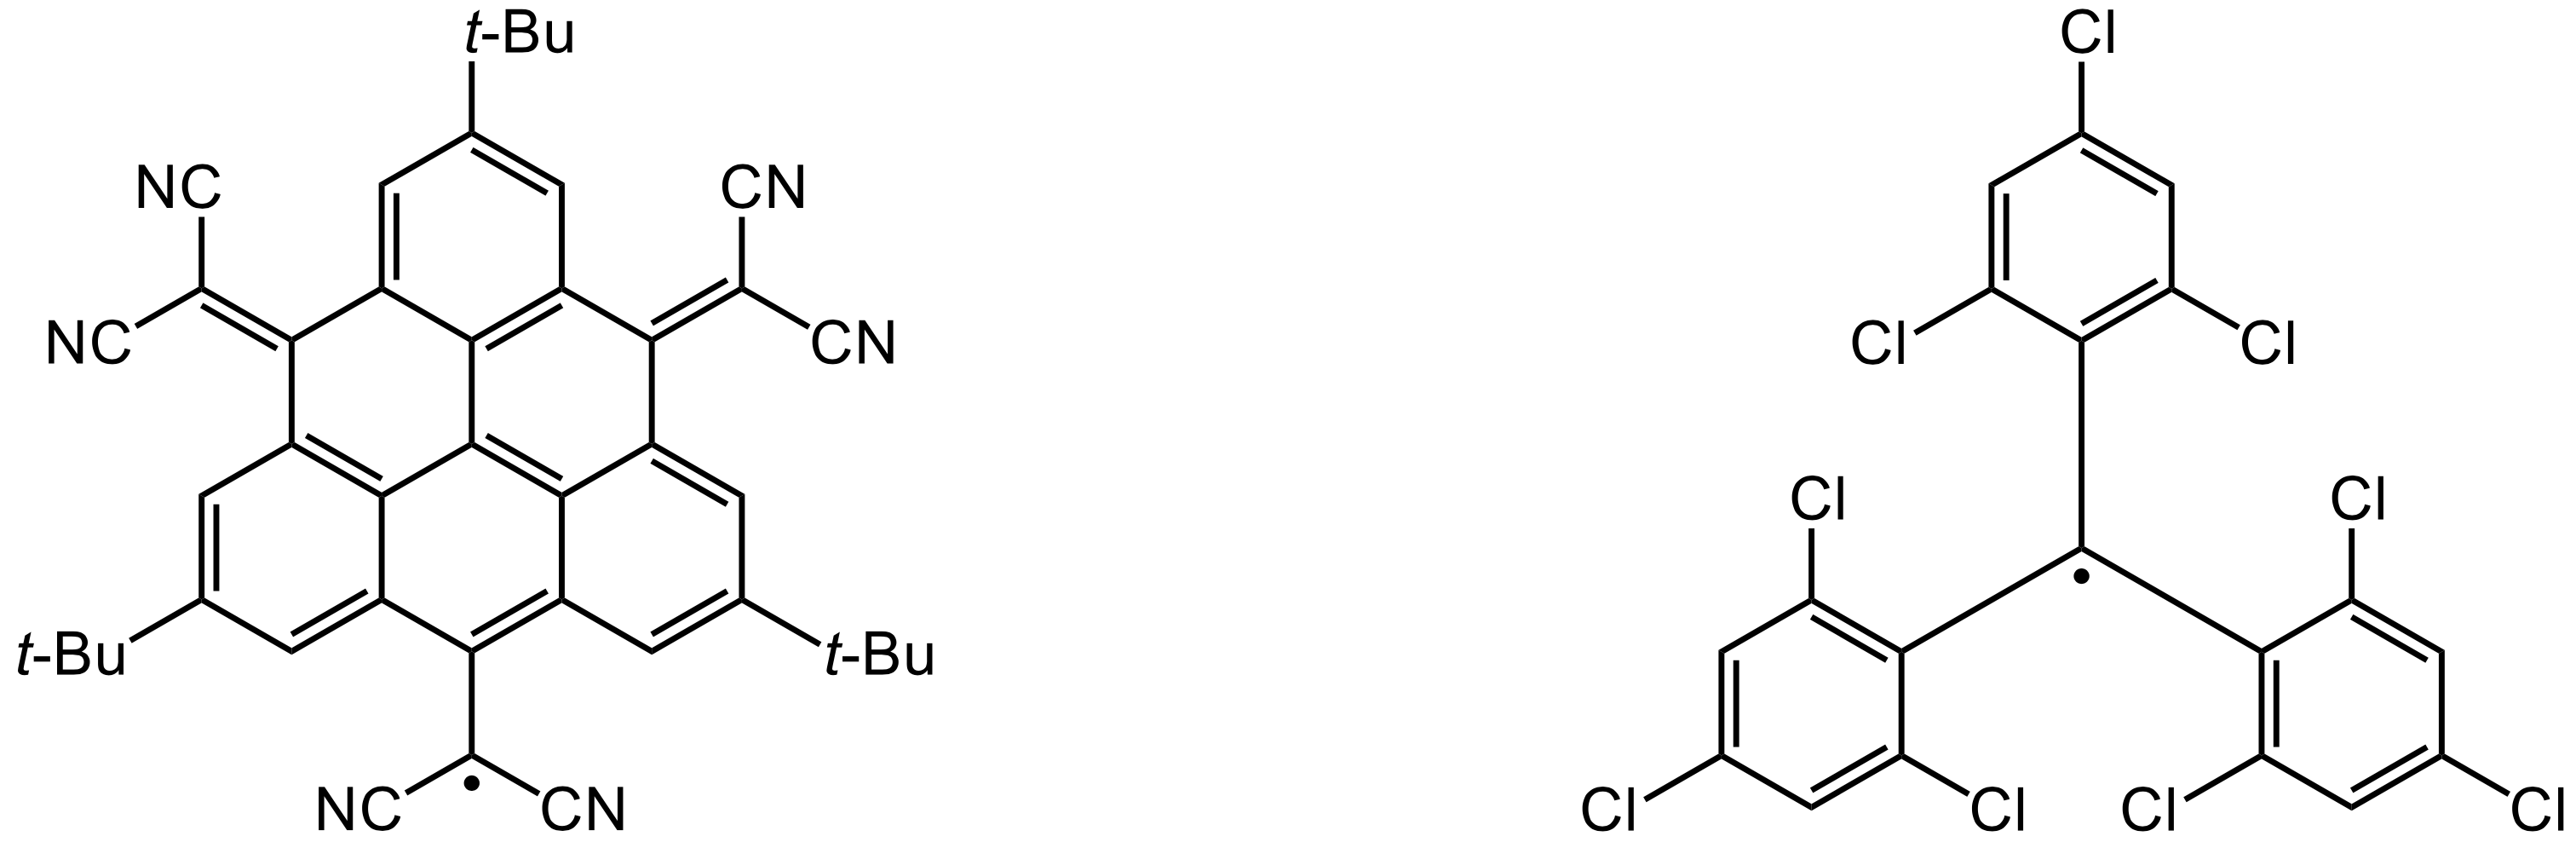
\includegraphics[width=0.8\linewidth]{PSet2F1.png}
    \end{center}
    \begin{proof}
        A bench-stable radical --- also known as a persistent radical --- is a radical that is thermodynamically high-energy (as all radicals are) but kinetically slow to react. Persistent radicals typically have some mixture of resonance stabilization and steric blocking.\par
        \underline{Left radical}: This radical has an \emph{extreme} amount of resonance delocalization among both the polycyclic $\pi$-system and the nitrile electron-withdrawing groups. By my count, resonance structures indicate that there should be partial radical character at 19 distinct atoms in the molecule. Thus, the spin density map should be so distributed that no one site has enough radical character to react in a kinetically efficient manner.\par
        \underline{Right radical}: Due to steric inhibition of resonance --- see \textcite[282]{bib:Anslyn} --- this radical cannot efficiently delocalize because the conformation of the trichlorophenyl rings in space (i.e., the "paddle wheel" topology) prevents full planar double bond formation. Thus, there is more radical character on the central carbon, as drawn. However, the paddle-wheel groups sterically block access to this site, once again preventing kinetic dimerization.
    \end{proof}
    \pagebreak
    \item 
    \begin{enumerate}
        \item Propose a reasonable arrow-pushing mechanism that explains the formation of the major product in the reaction below.
        \begin{center}
            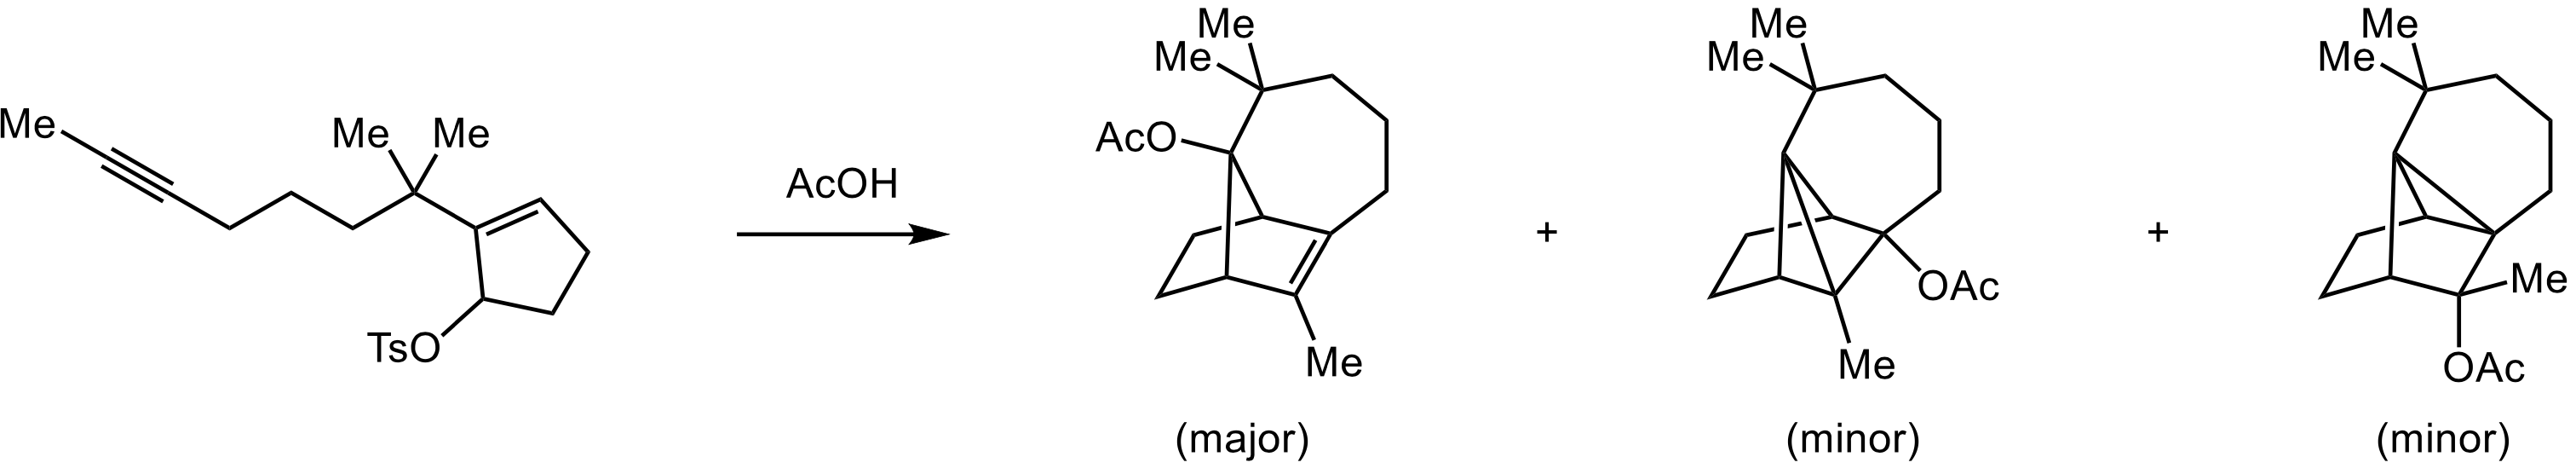
\includegraphics[width=0.95\linewidth]{PSet2F2.png}
        \end{center}
        \begin{proof}
            % The first intermediate could resonate (as an allylic cation) and react from either (symmetric) resonance structure; I've just drawn one resonance structure for simplicity.

            % Tosylate won't deprotonate acetic acid in solution because \emph{p}-toluenesulfonic acid is a stronger acid than acetic acid.

            % Intramolecular Gassman-type $[3+2]$ stepwise "cycloaddition" will outcompete nucleophilic attack. Can't be pericyclic because cationic $[3+2]$ is thermally forbidden.

            % $\pKa$ of acetic acid is 4.76, so it mostly exists in the protonated form in solution. Protonated acetic acid has $\pKa$ of $-6.1$, so tosylate is the stronger base.
            % $\pKa$ of \ce{TsOH} is $-2.8$.

            {\color{white}hi}
            \begin{center}
                \includegraphics[width=0.95\linewidth]{PSet2Q2a.png}
            \end{center}
            Due to its high degree of resonance stabilization, tosylate is a very good leaving group. Additionally, the cation created by a tosylate departure is both secondary and resonance-stabilized. As such, I propose that the reaction mechanism will be initiated by tosylate leaving. The majority of the tosylate ions in solution will then continue to exist as tosylate (instead of deprotonating acetic acid, for example) because tosylic acid is much stronger than acetic acid.\par
            Once the first intermediate is formed, it seems like it could do a cationic $[3+2]$ cycloaddition. However, such cycloadditions are thermally forbidden by the Woodward-Hoffmann rules (which we could also quickly see by drawing the HOMO of the alkyne and the LUMO of the allylic cation and observing the partial phase mismatch). As such, I propose that the allylic cation reacts intramolecularly via a two-step Gassman-type $[3+2]$ non-pericyclic "cycloaddition." Intramolecular "cycloaddition" would likely outcompete external nucleophilic attack both because it's an intramolecular process (greater local concentration), and there aren't any particularly \emph{great} nucleophiles in solution. Additionally, while I have drawn the first step proceeding from a particular resonance structure, in reality, either symmetric resonance structure could react to form the same ensuing intermediate.\par
            After the Gassman-type cycloaddition, a homoconjugation-stabilized cation will be left on the norbornene analog. This cation can then react with the best (and highest concentration) nucleophile in solution, which will be protonated acetic acid. Acetic acid has $\pKa=4.76$ (in \ce{H2O}), so it will likely largely exist in the protonated form regardless of the solvent in which we run this reaction. Theoretically, tosylate could also react in this step to add in, but there's much less of it, it's a much worse nucleophile, and we've already discussed in class how homoconjugation speeds up tosylate departure from that position in norbornene by 5-11 orders of magnitude; so even if tosylate did add in, that process would likely be highly reversible.\par
            Once acetic acid adds in, its proton will be highly acidic and easily deprotonated by a base in solution. This could be the solvent, but it could also be \ce{AcO-}, \ce{TsO-}, or \ce{AcOH}. Among these choices, I feel like \ce{AcO-} would do the deprotonation the most often because even though there's not much of it present, there will still be more of it than \ce{TsO-} (and it's more basic than \ce{TsO-}) and for \ce{AcOH2+}, $\pKa=-6.1$. This deprotonation yields the final product.
        \end{proof}
        \item Suggest how the minor products could be formed and draw the key intermediate(s) involved.
        \begin{proof}
            {\color{white}hi}
            \begin{center}
                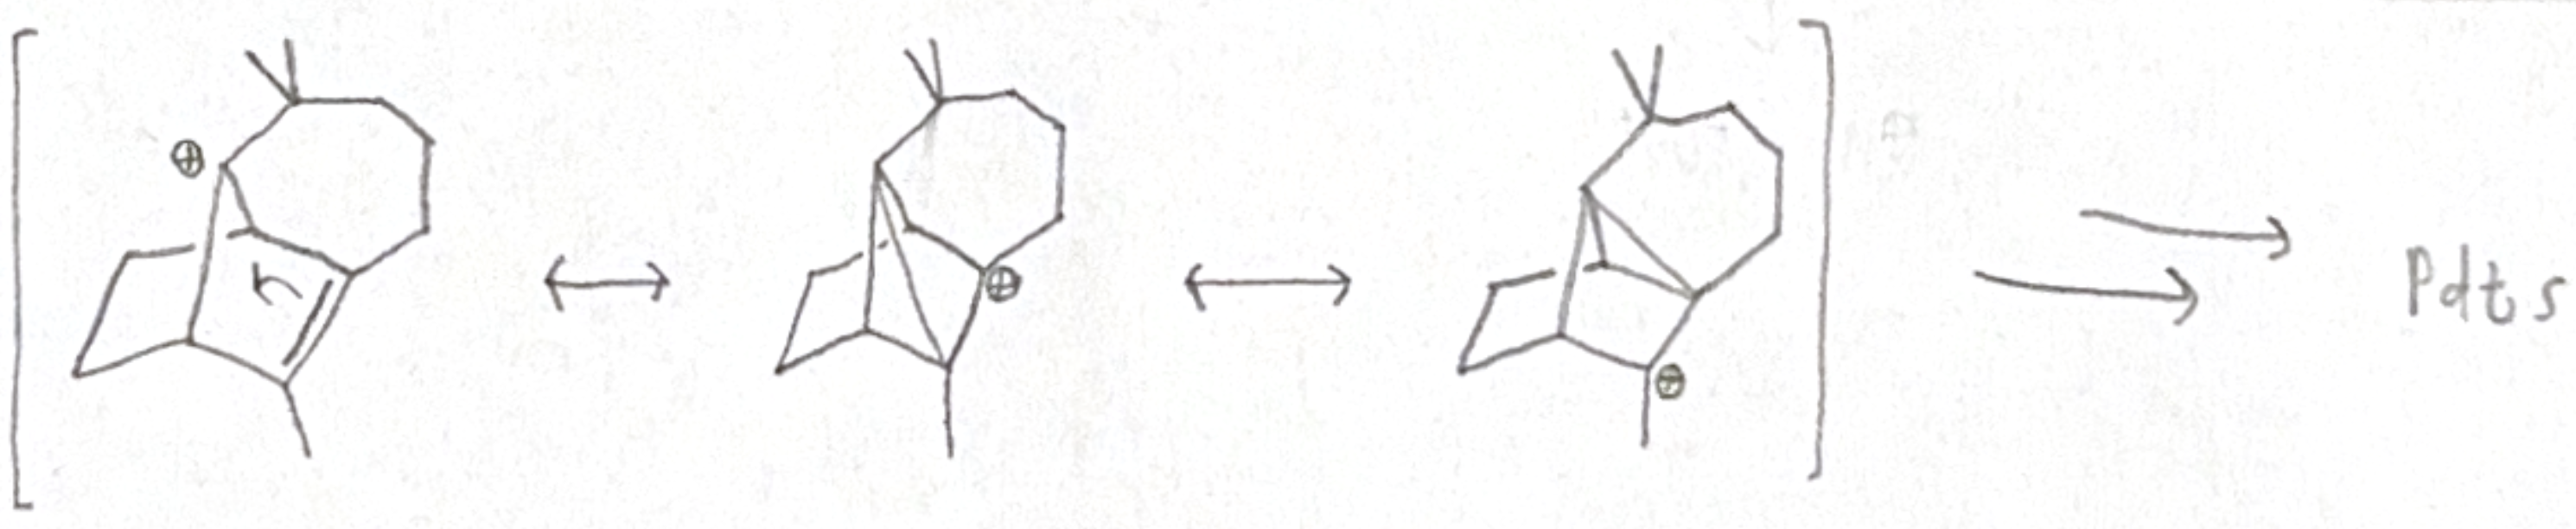
\includegraphics[width=0.85\linewidth]{PSet2Q2b.png}
            \end{center}
            I suggest that the final cation before \ce{AcOH} adds in has partial nonclassical, 3c-2e character. It will still favor the homoconjugation-stabilized form drawn in part (a) --- accounting for why that gives the major product --- but a Mulliken partial charge on the other carbons could also lead to \ce{AcOH} addition to those resonance forms followed by deprotonation, as drawn in part (a).
        \end{proof}
    \end{enumerate}
    \pagebreak
    \item Which of the following two compounds is more acidic (lower $\pKa$)? Compare the acidity of the protons indicated red. Rationalize your answer.
    \begin{enumerate}
        \item {\color{white}hi}
        \begin{center}
            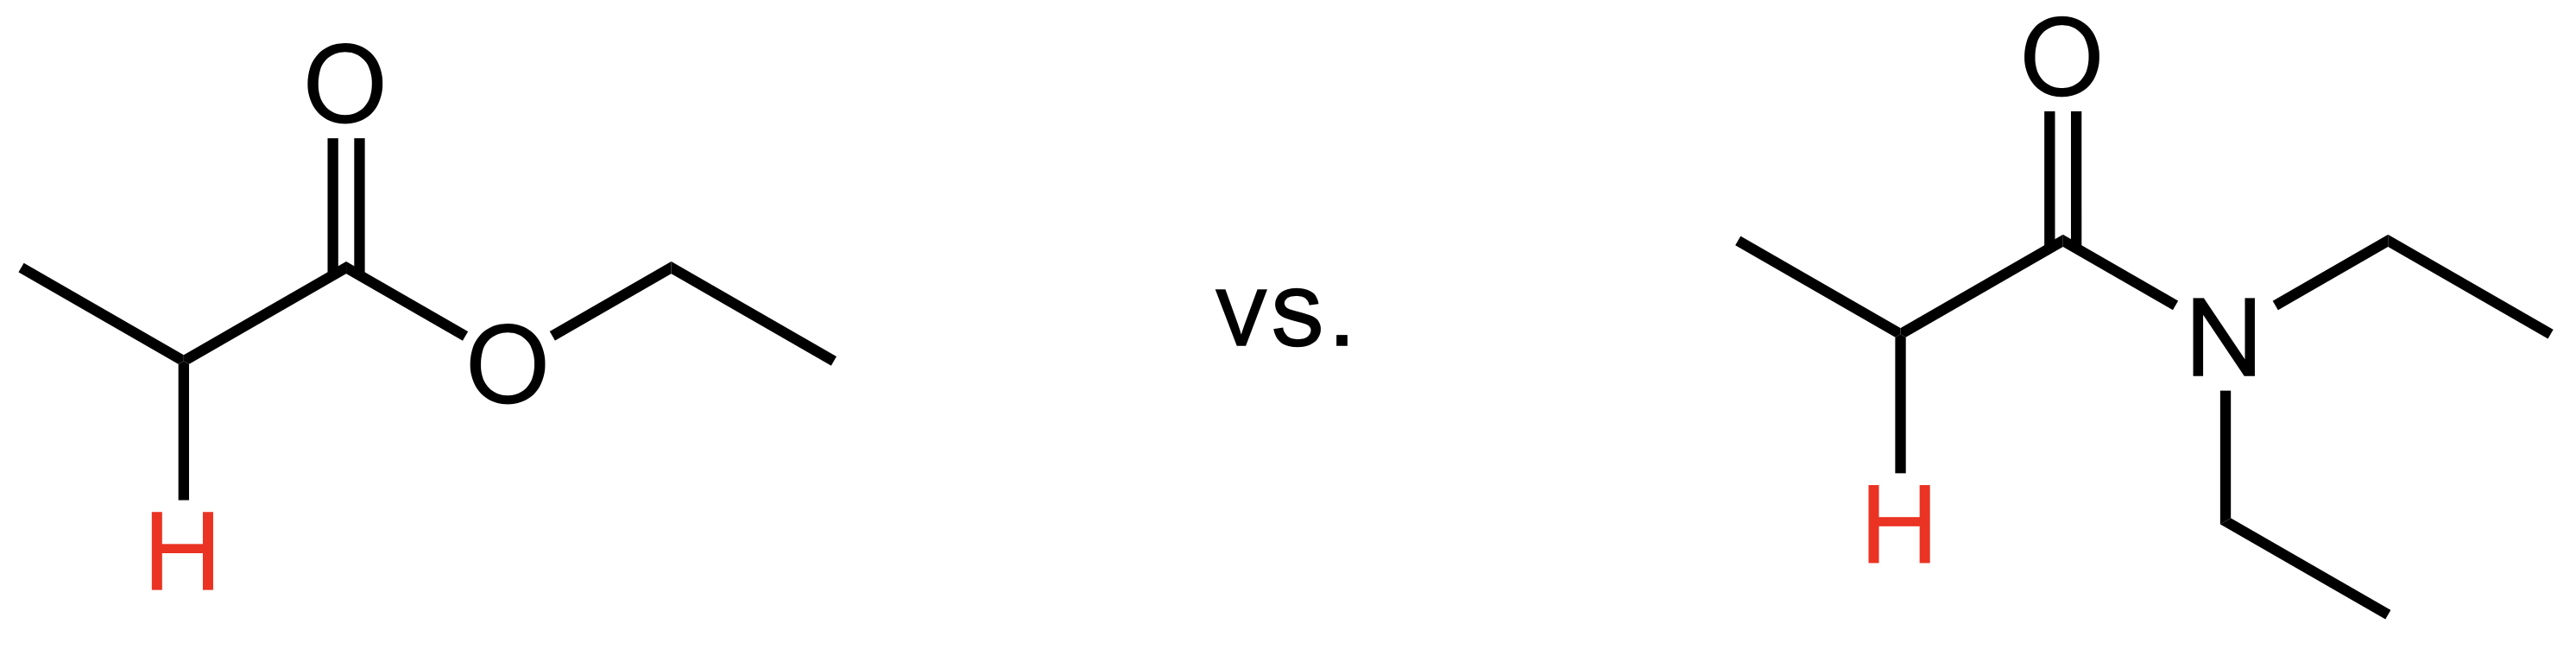
\includegraphics[width=0.45\linewidth]{PSet2F3.png}
        \end{center}
        \begin{proof}
            Neither esters nor amides are particularly enolizable since the lone pairs from the adjacent oxygen/nitrogen atoms compete with the resultant anion to delocalize into the carbonyl; this is an example of the resonance saturation effect described on \textcite[282]{bib:Anslyn}. However, \fbox{the ester will be more acidic} than the amide because the oxygen holds onto its electrons more tightly than the amide, thus sapping less of the carbonyl's potential ability to withdraw electrons.\par
            An alternative perspective to take is that the amide is more stable before deprotonation, and the two species have similar stabilities afterwards; therefore, it takes more energy to deprotonate the amide.
        \end{proof}
        \item {\color{white}hi}
        \begin{center}
            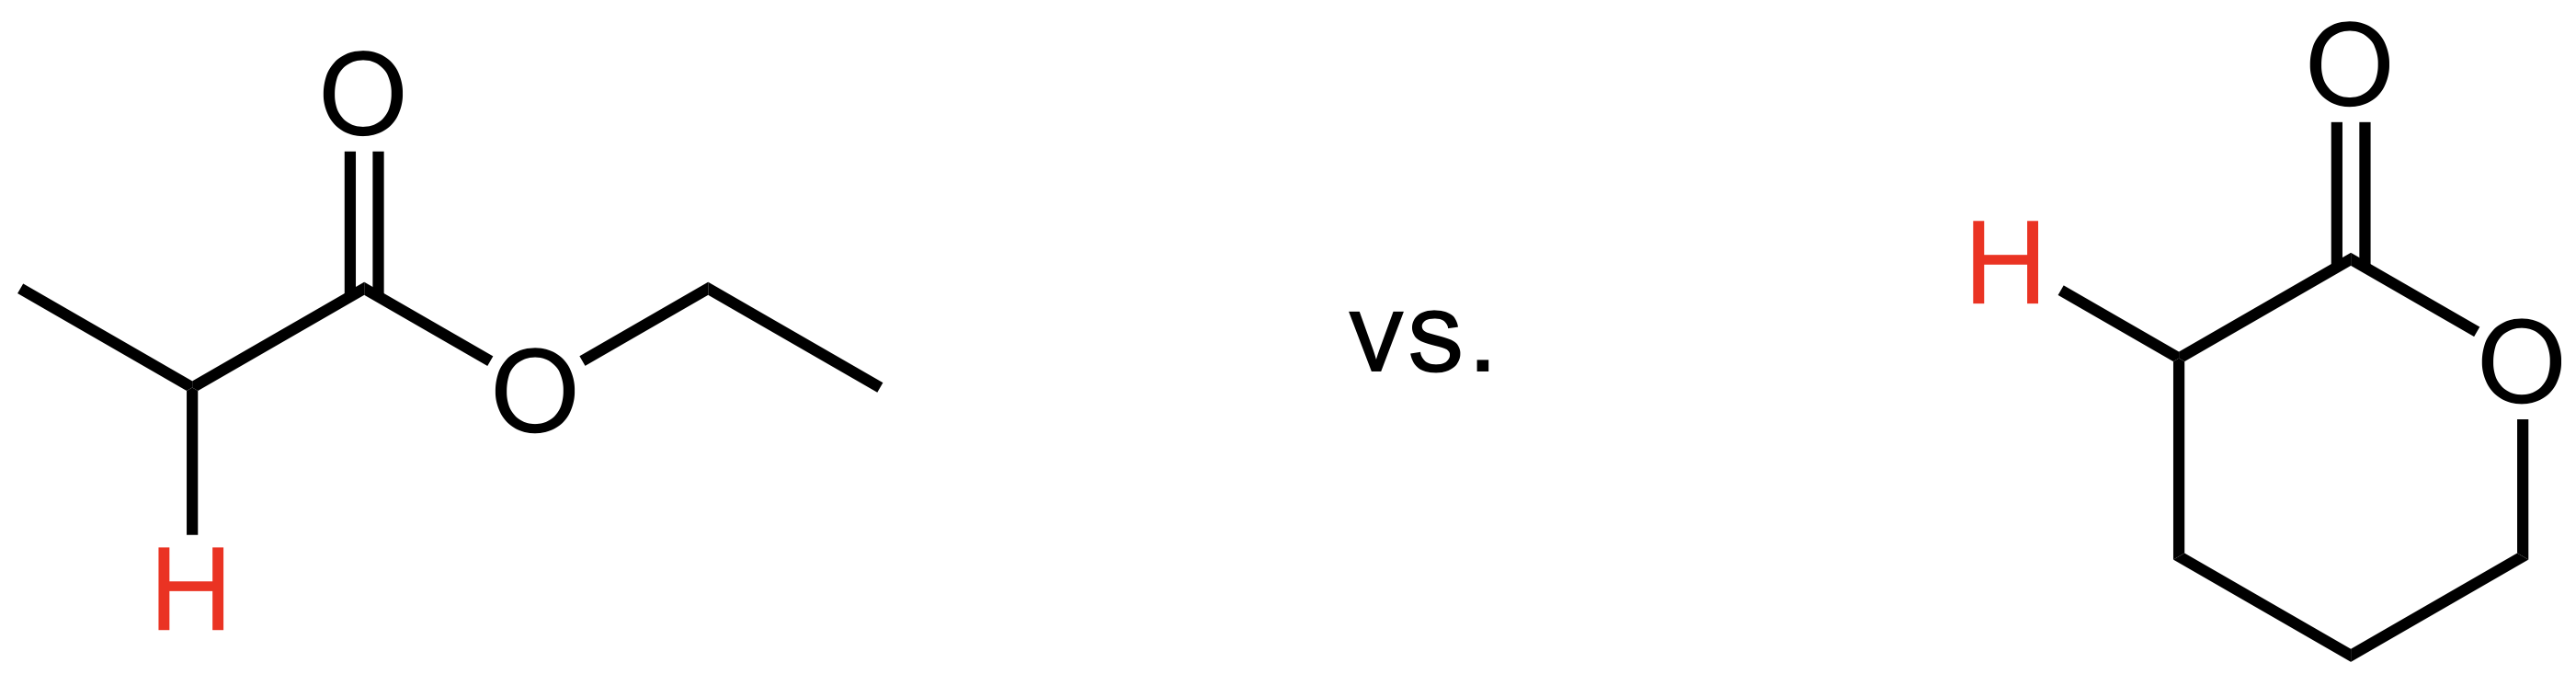
\includegraphics[width=0.45\linewidth]{PSet2F4.png}
        \end{center}
        \begin{proof}
            This regime is also governed by a resonance saturation effect. In both lactone and ester, the non-carbonyl oxygen will be $sp^2$-hybridized so that one of its lone pairs can conjugate with the carbonyl (specifically, the carbonyl's $\pi^*$-orbital). However, in the drawn conformation of the ester, the \emph{other} oxygen lone pair can \emph{also} delocalize through $n_{\ce{O}}\to\sigma_{\ce{C}}^*$ donation. This secondary interaction is not possible in the lactone, which is conformationally locked such that the other oxygen lone pair points away from the carbonyl's $\sigma^*$-orbital. The net effect is that the carbonyl in the lactone is less electronically saturated than the carbonyl in the ester, so the lactone anion can delocalize more effectively into the lactone carbonyl. But then the lactone can more readily stabilize the conjugate base, so \fbox{the lactone is more acidic.}\par
            We can also take the perspective that the lactone is more destabilized because the $n_{\ce{O}}$ dipole and the \ce{C=O} dipoles align and repel each other; the products, again, have similar stabilities.
        \end{proof}
    \end{enumerate}
    \pagebreak
    \item 
    \begin{enumerate}
        \item Suggest a reasonable mechanism for the following transformation.
        \begin{center}
            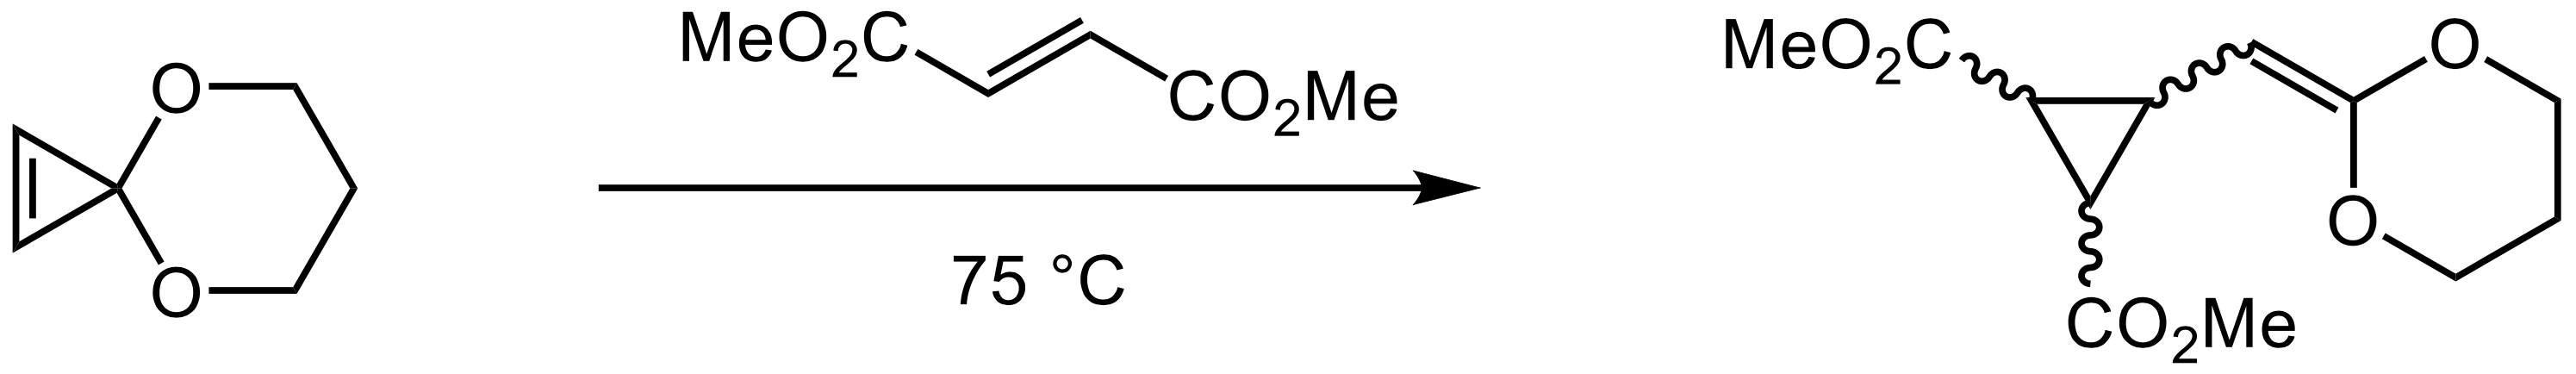
\includegraphics[width=0.7\linewidth]{PSet2F5.png}
        \end{center}
        \begin{proof}
            {\color{white}hi}
            \begin{center}
                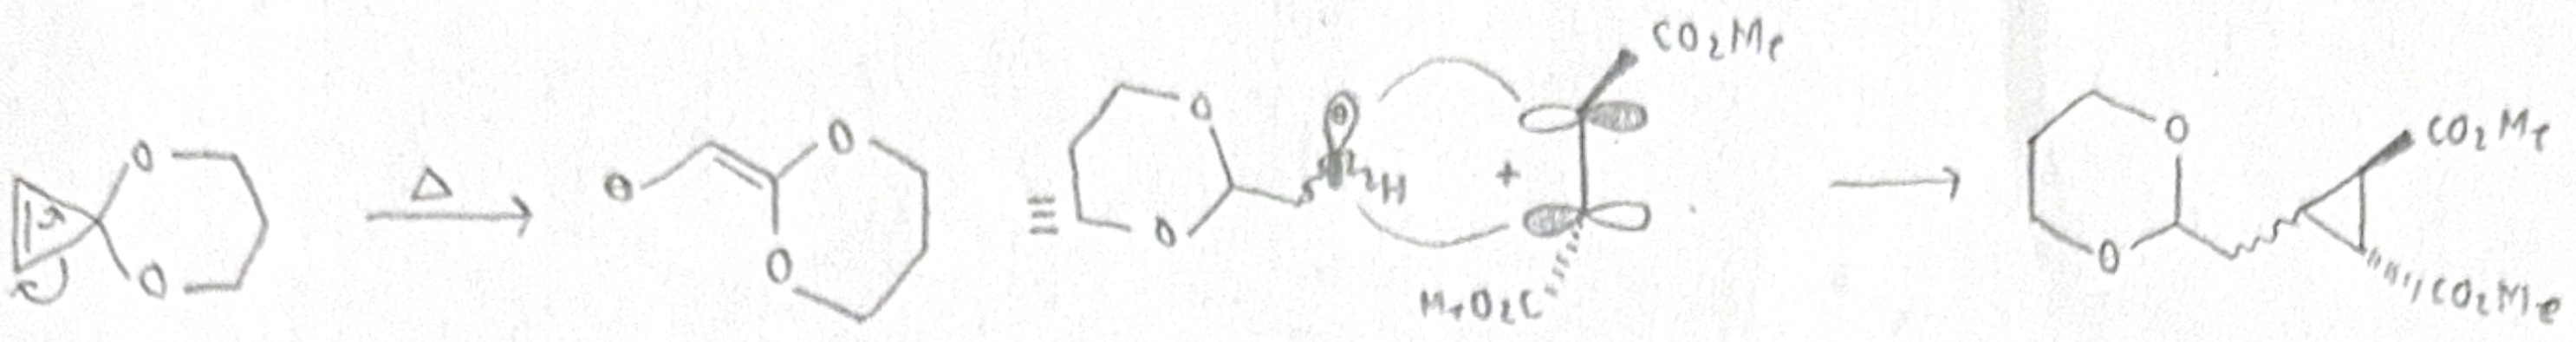
\includegraphics[width=0.95\linewidth]{PSet2Q4a.png}
            \end{center}
            The elevated temperature suggests --- as a first step --- either a homolytic bond cleavage (as in the case of AIBN) or some kind of pericyclic reaction. The cyclopropene bonds will likely be very strained, but all the same, the bonds will likely not be as weak as AIBN's bonds. As such, I propose a retro-anionic $4\pi$ electrocyclization as a first step. This will move the double bond to its final place and produce a \emph{singlet} carbene. Moreover, the carbene will remain a singlet because of the $\pi$-donor ability of the oxygen heteroatoms through the conjugated system. More accurately, when the oxygen atoms and $\pi$-system mix with the carbene \textbf{D}-orbital, they stabilize themselves and raise the energy of the empty \textbf{D}-orbital, making it more energetically favorable to pair electrons in the \textbf{C${}^{\bm{\prime}}$}-orbital. There would also be an argument to make --- based on class content --- that conjugation with the $\pi$-bond favors the triplet state, but I believe that the $\pi$-donor ability from two oxygens (as described above) will outweigh this competing effect.\par
            This singlet carbene can then be approached (on either face!) by the other reactant. I predict that the carbene will react with its HOMO since it is receiving electron density from a $\pi$-donor, while the other reactant will react with its LUMO since it has two adjacent ester EWGs. With the phasing match of a nonlinear approach, the next step will be a chelotropic $[2+1]$ cycloaddition, forming our product. The \emph{trans}-EWGs of the alkene will yield a \emph{trans}-product, but --- as mentioned above --- we will get some of both diastereomers with respect to the other bond because the carbene has two faces open to nonlinear approach.
        \end{proof}
        \item Discuss the stability of the intermediate(s) and predict the stereochemistry of the product.
        \begin{proof}
            See part (a).
        \end{proof}
    \end{enumerate}
    \pagebreak
    \item Draw potential energy diagrams for each of the following situations. Use dashed horizontal lines to indicate equivalent energy levels.
    \begin{enumerate}
        \item A single substrate can undergo two reactions with equal rates but different product stabilities. What reaction conditions would you use if you wanted a mixture of products? What reaction conditions would you use if you wanted a single product, and which product would you expect?
        \begin{proof}
            {\color{white}hi}
            \begin{center}
                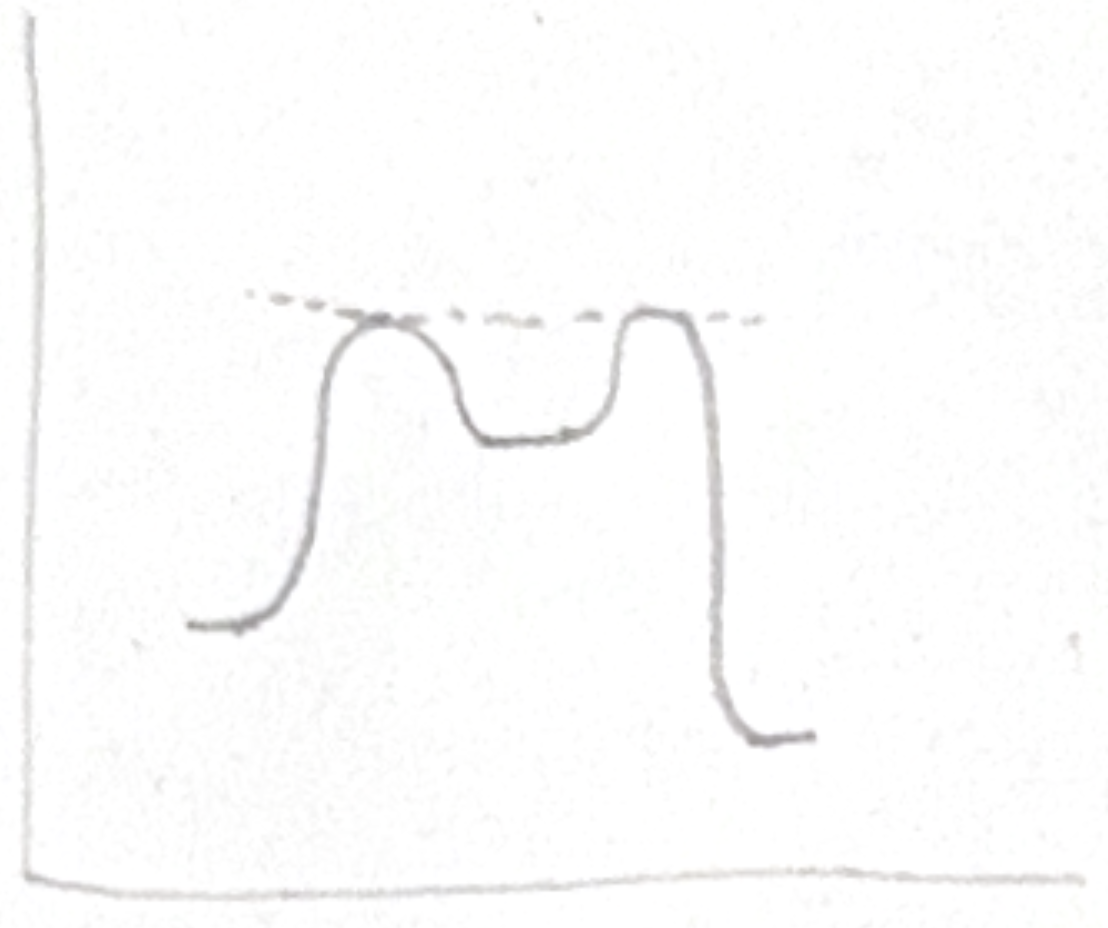
\includegraphics[width=0.4\linewidth]{PSet2Q5a.png}
            \end{center}
            Draw the substrate at an arbitrary energy level. Since both reactions have equal rates, draw humps with equal $\Delta G^\ddagger$ to both sides of it, one for each reaction. Then curve the humps down to products at different energy levels.\par
            If I wanted a mixture of products (i.e., the kinetic products irreversibly formed through the energetically equivalent transition states), I would use \fbox{short reaction times} and \fbox{low temperature.}\par
            If I wanted a single product (i.e., the thermodynamic product formed irreversibly along with a reversibly formed alternate product), I would use \fbox{long reaction times} and \fbox{high temperature.} It follows that I would expect the \fbox{more stable} product to be formed at the end.
        \end{proof}
        \item The formation of a kinetically stable radical from a precursor and dimerization of that radical.
        \begin{proof}
            {\color{white}hi}
            \begin{center}
                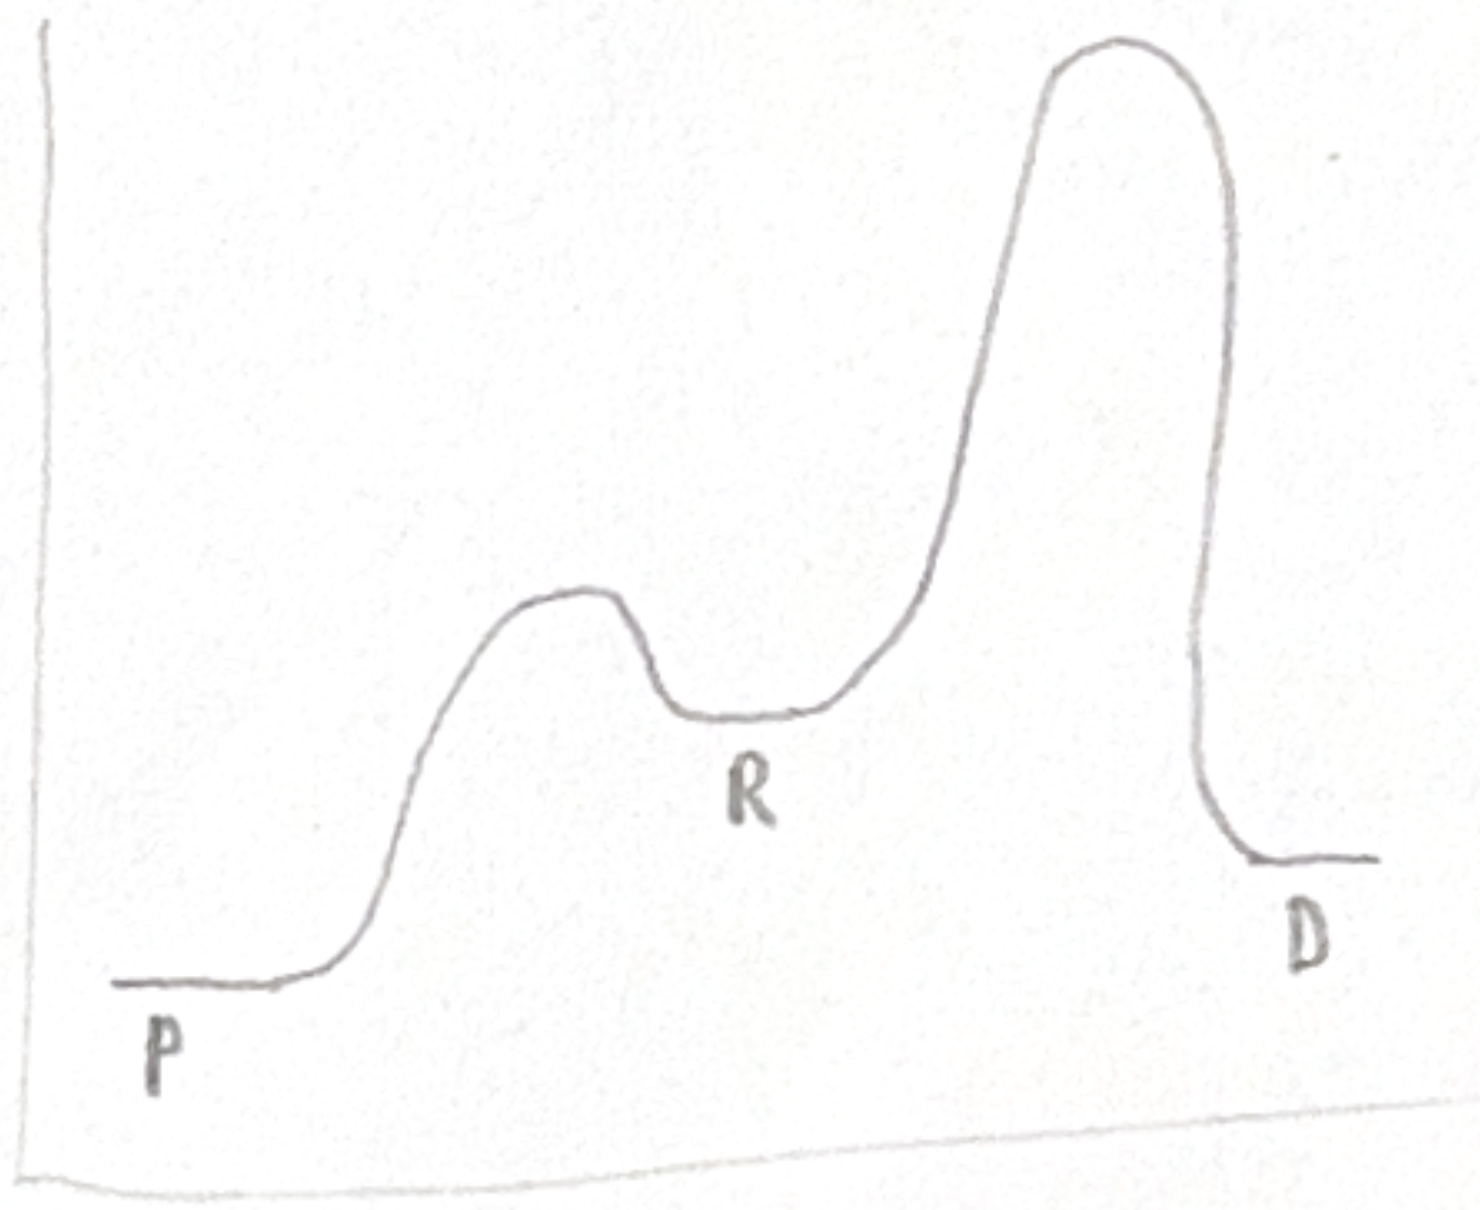
\includegraphics[width=0.4\linewidth]{PSet2Q5b.png}
            \end{center}
            The precursor (P) goes over a slight energy hump to become a relatively higher energy radical (R). Once the radical is isolated, it is kinetically stable, meaning that there must be a \emph{very} high energy barrier to it forming the dimer (D). Note that the dimer would still be more \emph{thermodynamically} stable than the radical (because persistent radicals are still \emph{radicals}; they don't want to exist). Also, we would probably need more information to determine \emph{for sure} whether the dimer or precursor is more thermodynamically stable, but I drew it higher in energy because I feel like in a number of systems (envisioning TEMPO, for instance), the steric blocking groups would seriously clash in a dimer, making it less thermodynamically stable than whatever precursor we're using (e.g., TMP).
        \end{proof}
        \item The stereoselective protonation of a tertiary carbanion.
        \begin{proof}
            {\color{white}hi}
            \begin{center}
                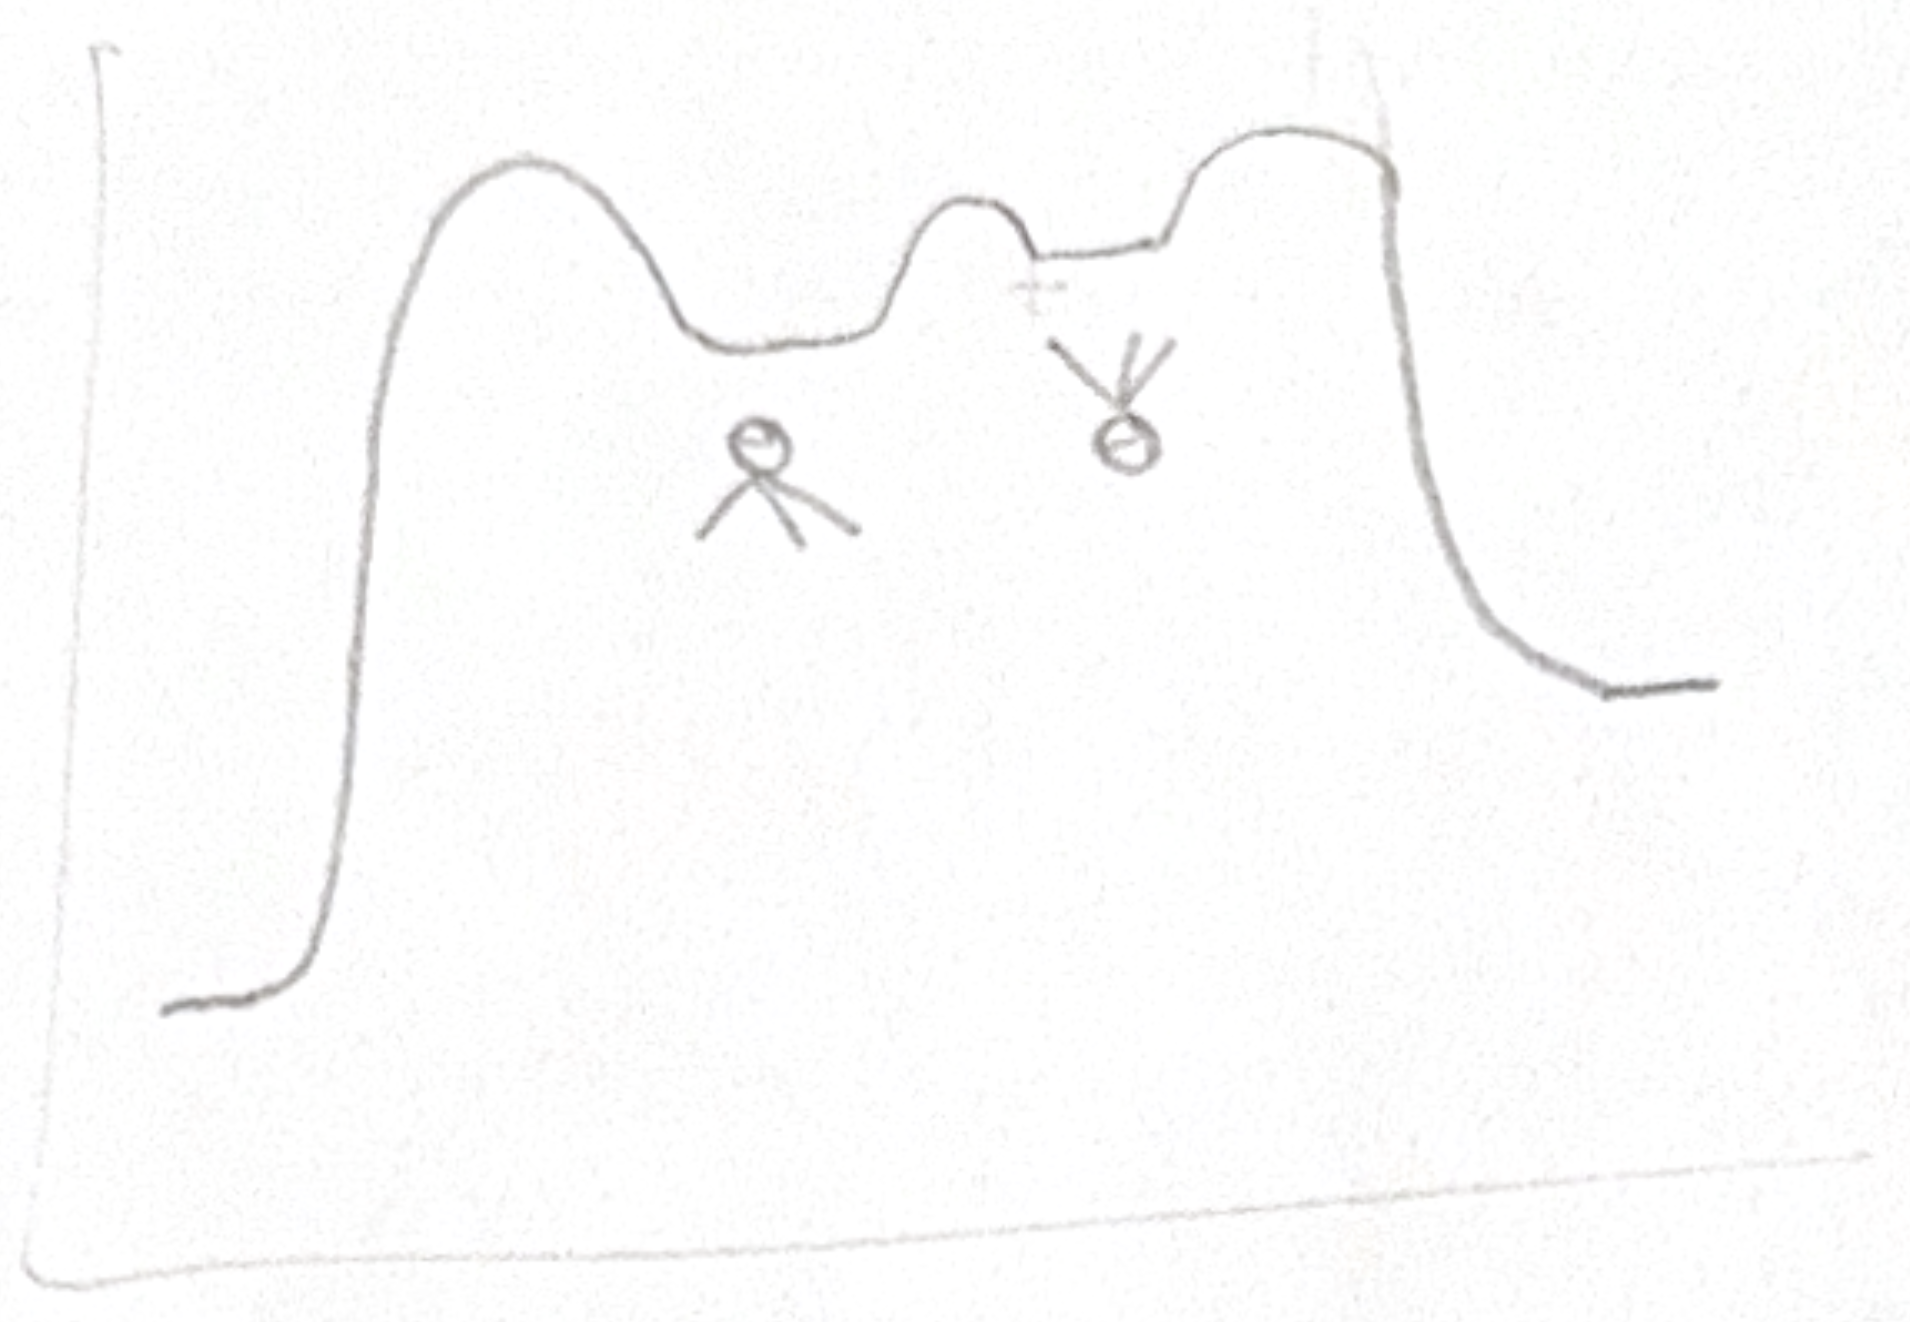
\includegraphics[width=0.4\linewidth]{PSet2Q5c.png}
            \end{center}
            Since it can generate two stereoisomers, the tertiary carbanion must be able to be protonated on either of its prochiral faces. As such, I propose a Curtin-Hammett regime in which the tertiary carbanion is in equilibrium between two inversion states. The inversion state that is slightly higher in energy will be the one that brings the more sterically bulky groups closer together. From here, we will have protonation that will likely be fairly low-barrier (as it gets rid of the reactive intermediate anion), and likely result in fairly equal-energy products. However, the higher energy anion will have its bulky groups closer together, meaning that the anion is more exposed for \emph{slightly} easier protonation, and it will also probably form the \emph{slightly} less stable product since, again, the bulky groups will be closer together. This is like Curtin-Hammett Scenario 2.
        \end{proof}
        \item Starting from one pure diastereomer, the epimerization of the alpha position of a ketone under acidic conditions to form a mixture of products.
        \begin{proof}
            {\color{white}hi}
            \begin{center}
                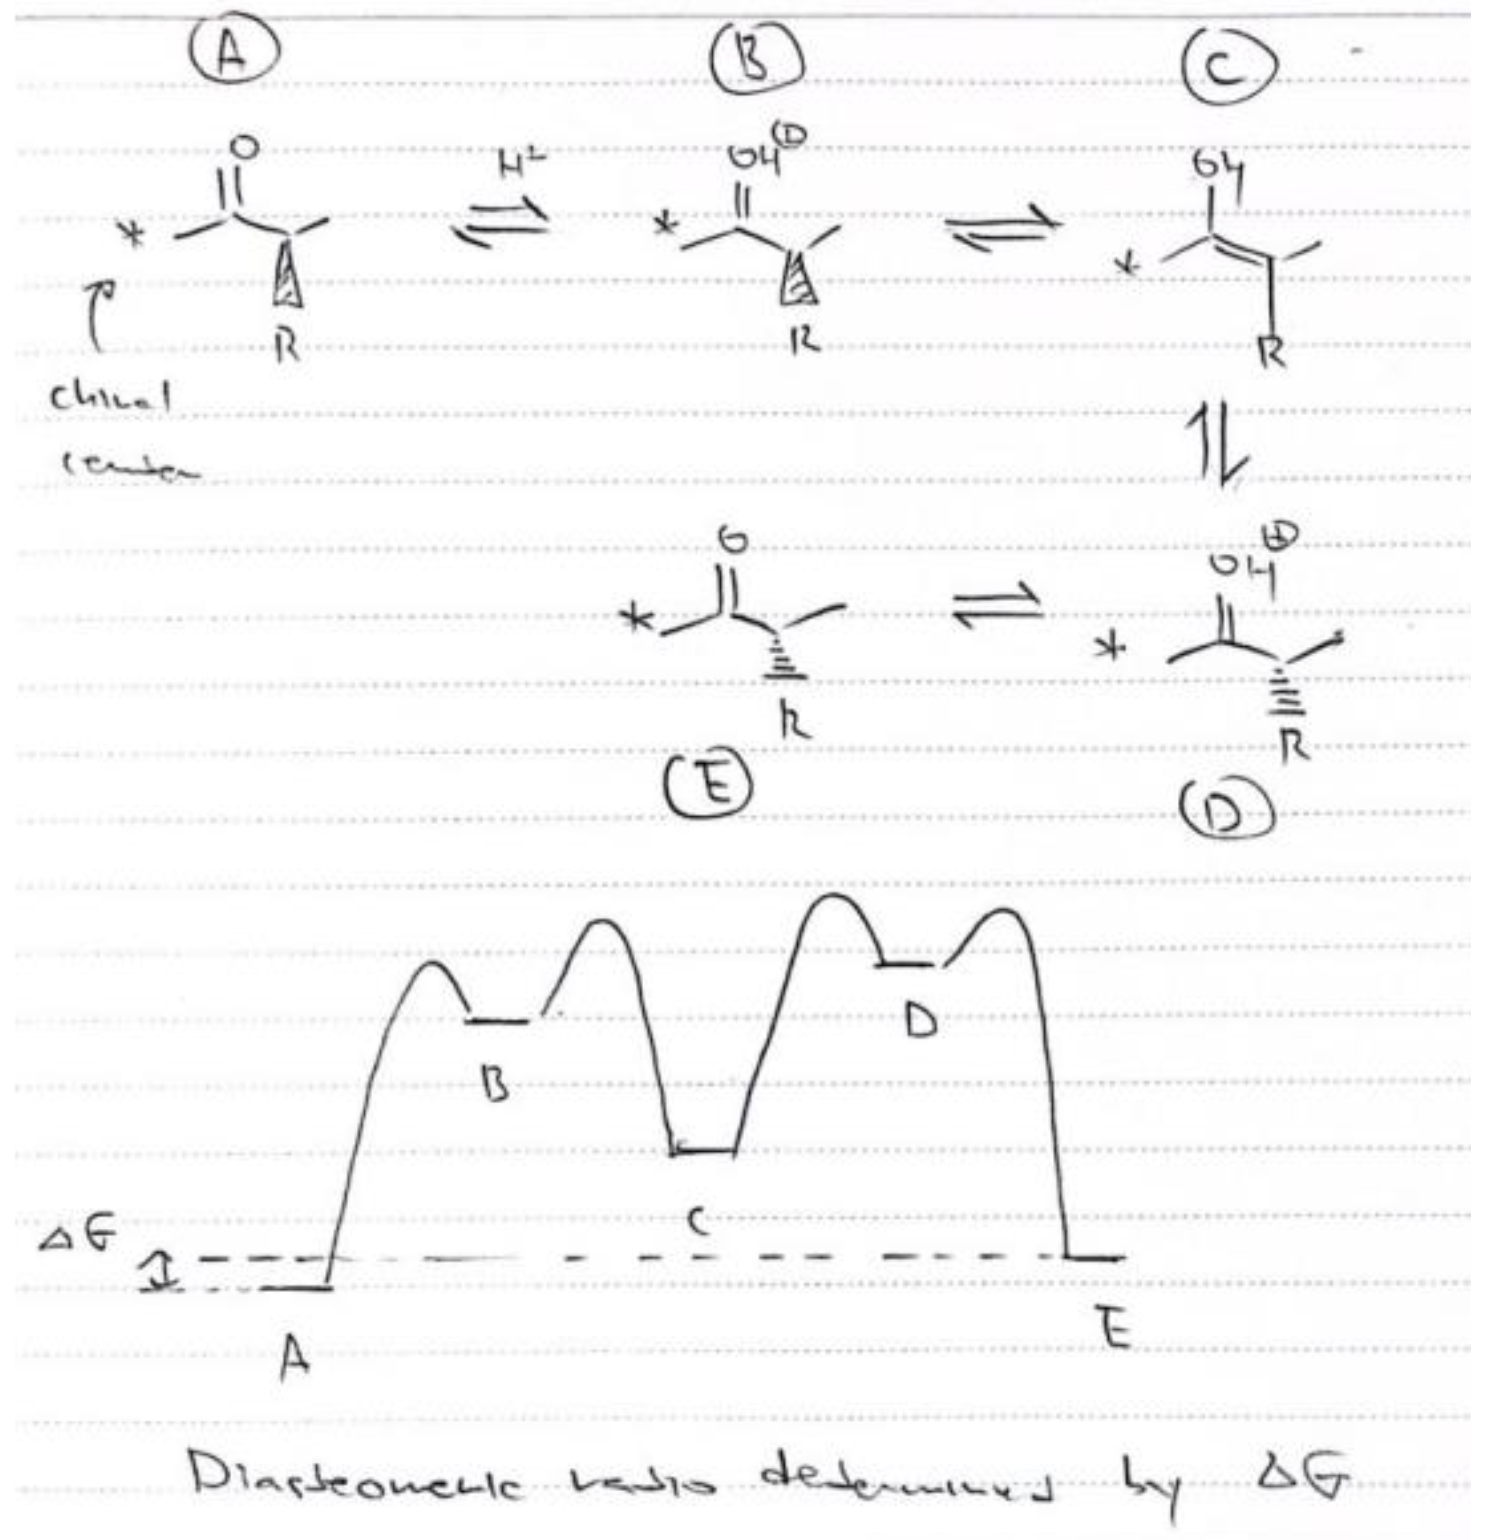
\includegraphics[width=0.65\linewidth]{PSet2Q5d.png}
            \end{center}
        \end{proof}
    \end{enumerate}
\end{enumerate}




\end{document}